
\section{Proposed Research Plan}

We now turn to the set of research
problems that will be addressed by the proposed project.

\subsection{Optimization of Very Large Computational Plans}

\noindent
\textbf{Problem description.}
A typical PC application builds up a graph of \texttt{Computation} objects (\texttt{JoinComp}, \texttt{SelectionComp}, etc.).  
This graph can be very large, especially for machine learning.  For example, 
processing a layer in a forward pass in a deep feedforward network can take five operations, with seven
in the backward pass.  Ten backpropagation iterations over a ten-layer network is more than one thousand operations.

PC relies on automatic, relational database-style optimization to choose the correct plan for such a computation.
Unfortunately, it is difficult to optimize very large graphs---performing logical optimizations such as 
changing join orders, as well as physical optimizations such as pipelining operations into one another and choosing implementation
algorithms.  Classical cost-based
relational techniques \cite{selinger1979access} break down after more than a few dozen operations \cite{graefe1993volcano}.
An obvious solution is to cut the graph into manageable pieces, and optimize and execute each piece separately.
The problem is that such a cut can be arbitrarily bad.  For example, in \texttt{LilLinAlg},
a multiplication of matrices \texttt{A} ($n\times m$ sub-blocks)
and \texttt{B} ($m\times p$ sub-blocks) 
produces $n \times m \times p$ blocks from a join, which is followed by an aggregation.  If pipelined into the aggregation, that set
of blocks is never materialized---it is streamed across the network and immediately aggregated.  
But if we are unlucky enough to cut the graph so as to separate the aggregation and the
join, we will materialize a huge intermediate result.  This is debilitating.

\vspace{5 pt} 
\noindent
\textbf{Proposed approach.}
We plan to formalize the problem of breaking a large computational plan into a set of \emph{frames}, or connected sub-plans.
Each frame is optimized and executed separately, and its output materialized.
It is possible
to write the problem of producing a ``good'' partitioning
as an integer program, where the goal is to produce a set of frames such that no frame exceeds an input maximum size.
This is done so as to minimize the value of a cost function that measures the cost incurred by the cut.
Different
costs are incurred by separating different types of operations.  Separating an aggregation from a subsequent operation
is generally low cost---aggregation tends to reduce output size, and it is blocking and cannot be pipelined. So forcing
such a result to be materialized is not often problematic.
But separating
a selection from either the operation before it or after it is high cost; it is always possible to pipeline though a selection, and
so cutting before or after a selection necessarily requires an un-necessary materialization.  

\vspace{5 pt}
\noindent
\textbf{Research Questions.}  There are several obvious research questions.  First, this particular IP formulation is NP hard.  Can
we develop heuristics to solve it effectively?  Also, how to choose the various weights?  They can be chosen through trial and error
or thought experiment and shipped with the system, but are there better methods?  Might we develop methods that can learn
over time?
What information should be passed across frames?  How do we recognize when an operation in one frame must have the same output
size as an operation in another frame?  In many ways, this resembles the query containment problem \cite{calvanese1998decidability, kolaitis1998conjunctive}.
Can we leverage the fact that, especially in machine learning computations, various patterns are repeated
iteratively?
That is, can we develop a method that uses already-observed information to improve the solution?

\subsection{Statistical Models for Combined Execution and Optimization}

\noindent
\textbf{Problem description.}
Classical, cost-based methods for optimizing computations do not necessary apply over opaque user code.
While PC may understand that
a particular operation such as a \texttt{JoinComp} is checking for equality across two sets (due to the programmer's
use of the \texttt{==} operation
in PC's Lambda calculus) and it will even understand where the values are coming from (an opaque C++ lambda, a method call, an attribute,
etc.), PC will \emph{not} have the key statistics, such as the number of unique values returned from an opaque C++ lambda, 
that are typically used for estimating the size of a join.  

\vspace{5 pt} 
\noindent
\textbf{Proposed approach.}
Optimizing in the face of this sort of uncertainty presents a classical exploration/exploitation tradeoff \cite{kocsis2006bandit}. 
One can  
execute a computation (or partially execute a computation) in order to obtain a set of statistics, and then optimize the 
remainder of the compute plan after obtaining the
statistics, or one can simply jump into the computation, and do the best job possible with the information at hand.  The former is
exploration, and the latter is exploitation.  Exploration has a cost, as stopping to plan means that opportunities for optimization,
such as pipelining, are lost.  We model the task of optimizing in the face of uncertainty as a 
Markov Decision Process (MDP) \cite{cassandra1998exact, white1991survey}.  Each state in the MDP consists of the portion of a computation that has been executed, the portion
left un-run, and the set of statistics that have been collected.  If one includes information such as a prior distribution over
the various statistics such as the number of distinct values, it is possible to compute the expected reward of moving to a new state 
by integrating over the value of each statistic.  However, this is computationally very difficult---even using Monte Carlo methods for
the integration \cite{littman1995complexity}---as it also requires optimizing the plan in the face of every possible value for the statistic.

As an alternative to solving the MDP precisely, we instead plan to apply deep reinforcement learning (deep RL) \cite{mnih2015human, lillicrap2015continuous, mnih2013playing} to the problem.  
Specifically, we will give the RL algorithm access to an encoding of the computational plan as well as the various statistics that
have been collected, the various choices for the next operation to run, as well as estimates for the cost of each of the operations,
as functions of the statistics.  By actually allowing the algorithm to make choices and execute parts of the computation and
then obtain feedback in the form of running time that is backpropagated through the network, the hope is that it is possible to
learn how to co-manage the collection of statistics and execution.

One of the fundamental problems with this approach is that RL can take a very long time to learn an effective policy, especially
in a rich environment.  It is likely impractical to actually learn
by running computations on top of PC, which can take a long time. 
Thus, our plan is to train
via 
simulation.  That is, we will build a simulator and synthesizer for synthetic computations that draws statistics from user-specified
priors, and use that to train the deep RL algorithm.

\vspace{5 pt}
\noindent
\textbf{Research questions.}  
Deep RL is often difficult to use in practice.
What exactly is th deep RL formulation?  How is the problem space to be encoded?  What do the deep networks look like?
Many formulas regarding the complexity of running
relational operations are known; how should those be incorporated into the RL?  
How does one synthesize reasonable computations for training the RL?

\subsection{Developing Support for Cross-Block References}

\noindent
\textbf{Problem description.}
One of the most important ideas in the design and implantation of PC is that all allocations are \emph{in place}, obviating the
need to ever serialize or deserialize PC \texttt{Object}s.  In order to support this, all PC \texttt{Handle}s by definition
point within a page, so \texttt{Handle} dereferences are always valid, even after a page moves across processes.
One difficulty is that cross block assignments often happen.  For example, we may have:
\texttt{Handle <Vector <Handle <DataPoint>}\texttt{>}\texttt{>} 
\texttt{myVec} \texttt{=} \texttt{makeObject <Vector <Handle <DataPoint>>> ();}.
By definition, \texttt{myVec} is now
stored in the thread's current allocation block.  Imagine that \texttt{storeMe} was
declared as \texttt{Handle <DataPoint>} and pointed to a PC \texttt{Object} that had just been read over the network.  The line of code
\texttt{myVec->push\_back (storeMe);}
will automatically deep copy the PC \texttt{Object} pointed 
to by \texttt{storeMe} to the current allocation block, preserving zero cost data movement.
When a deep copy fails due to lack of space, a fault occurs, the copy is undone, and the application (or, more likely, PC itself)
deals with the over-full page in an appropriate manner.

The problem with this is that sometimes, it is desirable to \emph{allow} cross-block \texttt{Handle}s.  
Always performing deep copies and forcing only within-block \texttt{Handle}s incurs a cost due to the copy.  It also seriously
limits the
size of an \texttt{Object} graph that a programmer can create, since graphs that are larger than a single page cannot be moved
across machines or to storage.  
Graph-based Big Data programming models have become popular, where programmers access data by traversing links, and we wish to 
support this.

\vspace{5 pt} 
\noindent
\textbf{Proposed approach.}
If one allows out-of-block \texttt{Handle}s, the key problem becomes dealing with faults efficiently.  
How does one ensure that when an out-of-page PC \texttt{Handle} is dereferenced,
the data it points to is accessed efficiently, perhaps across the network, without wasted CPU cycles? 
The key idea we wish to explore is \emph{latency masking}, closely related to the methods used in classical context switching \cite{silberschatz2014operating}.  
Because all PC computations logically operate in parallel over the items in a large set,
it may be possible to react to a fault 
by saving the state 
of the computation for the current PC \texttt{Object}, requesting the data transfer,
and moving onto the next \texttt{Object}. There is typically always another \texttt{Object} to process, 
and by definition, PC \texttt{Object}s can 
be processed in any order.  Each computation that causes
each fault is saved, and then resumed when the referenced \texttt{Object}'s page is retrieved.
Note that the key difference between this approach and classical applications of context switching that the contexts being saved
are within the same process and, in fact, the same thread---each context
is associated with the processing of a particular PC \texttt{Object}.

\vspace{5 pt} 
\noindent
\textbf{Research questions.} 
One key question is: is it possible to avoid such faults entirely by pre-fetching the targets of \texttt{Handle}s before they are
ever accessed?  Specifically, when a PC \texttt{Object} with a \texttt{Handle} is loaded into RAM, is it possible to develop a policy that
can be used to pre-fetch the \texttt{Object} in the background, before a fault occurs?
Also, since all PC computations are functional, they can be run and re-run without side effects (except for possible memory leaks
if the programmer uses C-style allocations).  This means that another option is simply killing the computation being run over an
\texttt{Object} when a fault occurs, loading the requested page, and then re-starting the computation, which will then run without fault.
This has the benefit that no state need be saved.
When to save context, and when to re-run?  

\subsection{Continuous Computations}

\begin{figure}[t]
  \begin{center}
    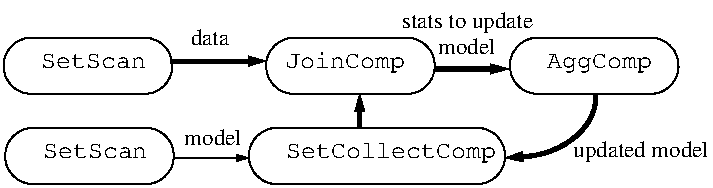
\includegraphics[width=4in]{ParamServer}
  \end{center}
\vspace{-10 pt}
  \caption{A parameter server using PlinyCompute.  Bolded links are those labeled as \texttt{continuous}.}
  \label{fig-param}
\vspace{-15 pt}
\end{figure}


\noindent
\textbf{Problem description.}
One of the most important applications for any distributed compute platform is machine learning, and
there is sometimes a significant
benefit to asynchronous computation in ML \cite{mnih2016asynchronous, dean2012large}.
Asynchronous computation may
result in models with lower error, as asynchronous training is less likely to over-fit the training data.  
Much work in asynchronous distributed machine learning utilizes
a distributed \emph{parameter server} architecture \cite{li2014scaling, ho2013more}, 
where a set of workers each request a subset of the current
model from a ``parameter server'' (essentially, a key-value store).  The workers then use that model 
to perform a computation over a subset of the data set; this computation updates the model and sends
the updated model back to the parameter server.  This update is asynchronous in that
workers may all be operating on different versions of the model, and updating the model without coordination.

The problem is that the programmer burden for writing a parameter server code is very high for anything other than
simple data-parallel computation where each worker operates on a separate copy of the model.  
Further, automatically-generated learning algorithms (such as those created by TensorFlow's automatic differentiation capabilities)
are unable to generate anything other than simple, data-parallel code when
often, complicated, model parallel implementations \emph{are} necessary.
Consider a large, deep neural network having 
two adjacent, fully connected layers of one million neurons.  This model requires a one-trillion entry
weight matrix.  Pushing
a batch of 100 data points through such a connection in one second
during training will require $2 \time 10^{14}$ FLOPS---the power in 20 high-end
GPUs---and the set of weights for an all-to-all connection will require more than a terabyte to store.
Such models must by definition be handled in parallel, but
developing such a code for a parameter server
is difficult at best.

Fortunately, orchestrating complex distributed computations of this sort on PC is quite easy.  Learning the weights
in the sort of application described above requires what amounts to distributed linear algebra, which is easy to implement on top of PC.

\vspace{5 pt} 
\noindent
\textbf{Proposed approach.}
That said, PC is purely a synchronous system.  To add asynchrony,
we will allow a programmer to label an output from one or more computations to be  
\texttt{continuous}.  Just like their non-continuous
versions, each
continuous computation represents a computation that produces a set of PC \texttt{Object}s.
However, the key difference is that a \texttt{continuous}-labeled 
computation is free to send any output \texttt{Object} computed from its current inputs
at any time.
This means that a \texttt{continuous}-labeled computation is forever updating and re-sending output \texttt{Object}s.

Each computation producing a \texttt{continuous}-labeled output must declare a key for the output \texttt{Object}s.  When
two output \texttt{Object}s with the same key are processed by any computation, the newer PC \texttt{Object} is removed, and the computation consuming
that set is responsible for updating its own output set with the new \texttt{Object}.  This update is asynchronous in the sense that
all computations are constantly updating their output sets in response to changes in their input, with no synchronization.

It is easy to simulate an asynchronous 
parameter server using these abstractions, as depicted in Figure \ref{fig-param}.  In this computational plan, data are
scanned continuously.  At the same time, the model is scanned into a \texttt{SetCollectionComp} and then joined with the 
data.  The computation that occurs in the \texttt{JoinComp}
corresponds to the computation done in a worker in a parameter server.
In the join, a set of statistics needed to update the model
are computed and aggregated---the result of the aggregation is the updated model.
As the updated model enters into the \texttt{SetCollectionComp}, it asynchronously replaces the initial model.  The current
state of the model is constantly re-sent into the join.  The cycle
repeats until convergence.

The benefit of this computation-centric view is that it is possible to build
complex computations with little effort.  A model-parallel computation---where a very large model is distributed across the cluster
is easily implemented.  For example,
a forward-backward pass through a deep network utilizing a series of distributed matrix multiplies corresponds
to a series of \texttt{JoinComp}--\texttt{} pairs.

Note that this looks a lot like continuous or stream-based query processing in database systems.  The key difference is that rather
than processing queries over sliding windows (as is typical in stream-based processing), query processing is done over constantly
updated sets.

\vspace{5 pt}
\noindent
\textbf{Research Questions.}  Building such functionality into PC will be challenging.
One key research challenge is how to efficiently perform online updates to query result sets---this looks
something like the materialized view maintenance problem from database systems \cite{gupta1995maintenance, agrawal1997efficient}.  We will investigate how to attach lineage 
to cached results \cite{buneman2007provenance, widom2004trio}, in order to efficiently perform the required updates, and
leverage ideas from streaming systems \cite{zaharia2013discretized, babcock2002models}  and continuous query processing \cite{chandrasekaran2003telegraphcq, chen2000niagaracq}.
Another challenge is how to develop reasonable algorithms
for scheduling and
resource management---especially memory management---which
will be difficult since all operations in a plan are potentially active at the same time.  

\subsection{Developing PC-Specific Compiler Optimizations}

\noindent
\textbf{Problem description.}
As a final research problem, we will attempt to develop a set of compiler optimizations 
(over the LLVM IR \cite{lattner2004llvm}) that are
specific to PC.  Through experience, we have found that there 
are a number of performance errors that PC programmers make that could be fixed by a compiler, if the compiler were
aware of the semantics of PC computations.  For example,
in PC, dynamic method call dispatch over PC \texttt{Object}s (and in, fact, all automatic movement and dynamic loading 
of code in PC)
is facilitated by the type code stored within each
\texttt{Handle} object.
The
type code is a unique identifier for the PC-\texttt{Object}-descended type of the object that the \texttt{Handle} points to.

In every major C++ compiler (GCC, \texttt{clang}, Intel, and Microsoft), virtual functions
are implemented using a virtual function table, or \texttt{vtable} object, a pointer to which is located at the beginning
of each C++ object having a virtual function.  Unfortunately, the \texttt{vtable} pointer is a native, C-style pointer, and so the
\texttt{vTable} pointer does not automatically translate when an
object is moved from process to process.  To handle this, in
PC's C++ binding, whenever a PC \texttt{Handle} object is dereferenced,
a lookup on the
type code is performed transparently to the application programmer, and the \texttt{vTable} pointer in the PC \texttt{Object} is ``fixed''.
First, if necessary, a shared library containing 
the correct \texttt{vTable} is fetched from PC's catalog server and loaded into RAM, and then the  \texttt{vTable} pointer
in the PC \texttt{Object} is changed to point to the correct \texttt{vTable}.

The problem is that since the code associated with a \texttt{Handle} deference cannot be sure of its context---whether it must
have already been dereferenced---this lookup must happen at \emph{every} dereference.  Programmers often put such dereferences
with a loop, as they assume the dereference is costly. We find that sometimes, these lookups
can take up 30\% of the CPU cycles in a PC computation.

\vspace{5 pt} 
\noindent
\textbf{Proposed approach.}
A careful programmer can re-factor code to avoid multiple dereferences, performing the dereference once before entering the loop,
leading to a dramatic increase in performance.  However, even though the target programmer for PC is a capable systems developer,
this
is asking a lot of a programmer.  It would be much better for the compiler itself to recognize such situations, and to take
appropriate action.  There are many other, similar optimizations that could catch and remedy standard PC programming errors.
Our plan is to implement these optimizations as an LLVM plug-in.

\vspace{5 pt}
\noindent
\textbf{Research questions.} Our experience tells us that there are many such examples of optimizations that could help fix many
of the problems that users have when attempting to use the PC \texttt{Object} model effectively.
What is the set of PC-specific compiler optimizations that can remedy common performance problems?
Might we change the semantics of PC computations to allow more opportunities for optimization?

\subsection{Evaluation}

All of the ideas explored as part of the proposed research project will be implemented and evaluated as part of PC; any
ideas that prove to have merit will be released as part of PC. To
measure our progress,
we will also develop a set of benchmark codes on top of PC, in three categories: machine learning,
data processing, and linear algebra (a preliminary version of this benchmark was described in the Preliminary Experimental Evaluation
section of the proposal).  In machine learning, we have already begun porting TensorFlow \cite{abadi2016tensorflow} onto PC, using PC's execution engine
rather than TensorFlow's own parameter server; we will maintain a number of deep learning benchmarks comparing PC to the current
release of TensorFlow; we will also maintain current
results comparing LDA, Gaussian mixture modeling, K-means, and several other standard
machine learning algorithms to implementations on top of Spark and Flink.  In data processing, we will continue to develop
various queries on the denormalized TPC-H data set, and compare with Spark and Flink implementations.  And finally, we will
continue to develop \texttt{LinLinAlg}, and maintain results comparing its speed with \texttt{MLLib}, SystemML, and SciDB.


